\documentclass{standalone}

\usepackage[OT1]{fontenc}
\renewcommand*\familydefault{\sfdefault}
\usepackage{helvet,sfmath}
\usepackage{siunitx}

\usepackage{tikz}
\usetikzlibrary{arrows,calc,patterns}
\usepackage{tikz,tkz-euclide}


\definecolor{BlueDefault}{rgb}{0.2,0.2,0.7}

\begin{document}

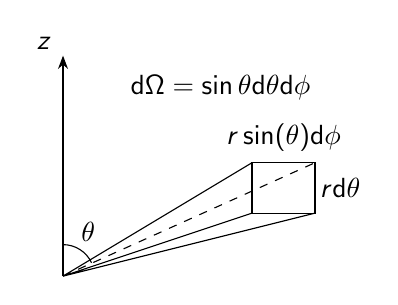
\begin{tikzpicture}[scale=0.8]
    \draw 
    (0,0) to (3,1)
    (0,0) to (4,1)
    (0,0) to (3,1.8)
    ;
    \draw[dashed]
    (0,0) to (4,1.8)
    ;
    \draw
    (3,1) to (4,1) to (4,1.8) to (3,1.8) to (3,1)
    ;
    \draw
    (3.5,2.2) node{\(r \sin (\theta) \mathrm{d} \phi\)}
    (4.4,1.4) node{\( r \mathrm{d} \theta\)}
    (2.5,3) node{\( \mathrm{d} \Omega = \sin \theta \mathrm{d} \theta \mathrm{d} \phi \)}
    ;
    \draw[-Stealth] (0,0) to (0,3.5);
    \draw (0,0.5) arc(90:25:0.5);
    \draw
    (-0.3,3.7) node{\(z\)}
    (0.4,0.7) node{\(\theta\)}
    ;
\end{tikzpicture}    

\end{document}